\documentclass{report}
\usepackage{graphicx}
\usepackage{titlesec}
\usepackage{longtable,booktabs}
\usepackage[left=2.54cm, right=2.54cm, top=2cm]{geometry}
\usepackage{enumitem}
\setlistdepth{9}


\titleformat{\chapter}{\normalfont\huge}{\thechapter.}{20pt}{\huge}
\titlespacing*{\chapter}{0pt}{0pt}{30pt}

\providecommand{\keywords}[2]
{
  \small    
  \textbf{\textit{#2---}} #1 
}

\begin{document}


\title{Introduction to \LaTeX{}}
\author{Author's Name}

\maketitle
\tableofcontents


\chapter*{Resumen}
\addcontentsline{toc}{chapter}{Resumen}


\vspace{-5mm}
Según la OMS, un destino médico es un cambio en el estado de salud de un invididuo, colectivo, o población, atribuible a intervenciones determinadas. La predicción de destinos médicos es una rama de la investigación médica que estudia el resultado final de la estructura y procesos del sistema médico en la salud y el bienestar de pacientes y poblaciones. Es un pilar importante en la toma de decisiones y en análisis de políticas y procedimientos, ya que permite la evaluación de la calidad del cuidado médico, su eficiencia y efectividad. Su objetivo es identificar fallos en la práctica médica que afectan a la salud del paciente y desarrollar estrategias que mejoren el cuidado. Para ello, mide eventos tangibles experimentados por el paciente, tales como la mortalidad, la readmisión o la morbilidad. El resultado de la investigación sobre destinos médicos se utiliza para informar a los cuerpos legistlativos que toman decisiones realacionadas con la sanidad, así como a órganos financieros, tales como el gobierno o compañias aseguradoras, que buscan minimizar costes médicos proporcionando un cuidado médico adecuado. La recolecta estandarizada de estadísticas y datos médicos acerca del cuidado médico que reciben los pacientes ha permitido que los registros médicos puedan ser empleados como una fuente fiable para la investigación.


Uno de los destinos médicos más relevantes es la mortalidad extrahospitalaria de los pacientes, es decir el tiempo hasta su defunción tras el alta hospitalaria. El objetivo de este estudio es la predicción de esta variables mediante redes neuronales artificiales. En concreto, se trata de una tarea de la predicción clasificatoria en tres franjas temporales (0 - 1 meses, 1 - 12 meses, 12+ meses). Para ello se emplean un total de 43 variables predictorias, incluyendo información demográfica, señales fisiológicas, resultados de pruebas de laboratorio y otras variables relacionadas con la estáncia hospitalaria de los pacientes. Obtenemos la información necesaria de la base de datos pública MIMIC-III v1.4, correspondiente a los ingresos hospitalarios en unidad de cuidados intensivos en el hospital Beth Israel Deaconess Medical Center, en Boston, Massachussets, EE.UU. Se trata de un conjunto de datos que contiene información médica deideintificada sobre más de 40.000 pacientes críticos entre los años 2001 y 2012. De esta forma, diseñaremos una red neuronal capaz de predecir satisfactoriamente la mortalidad extrahospitalaria de los pacientes en función de estas variables.
\vspace{5mm} 

\keywords{Redes Neuronales Artificiales, minería de datos, Inteligencia artificial, Predicción de mortalidad, aprendizaje profundo, Unidad de cuidados intensivos}{Palabras Clave}

\chapter*{Abstract}
\addcontentsline{toc}{chapter}{Abstract}
\vspace{-5mm}
According to WHO, a medical outcome is a change in the health status of an individual, group, or population, attributable to certain causes. The prediction of medical outcomes is a branch of medical research that studies the final result of the structure and processes of the medical system in the health and well-being of patients and populations. It is an important factor in decision making and analysis of policies and procedures, since it allows the evaluation of the quality of medical care, its efficiency and effectiveness. Its objective is to identify faults in medical practice that affect the health of the patient and the development of strategies that improve care. To do this, it measures tangible events experienced by the patient, stories such as mortality, readmission or morbidity. The result of the research on medical destinations is used to inform the legal bodies that make decisions related to health, as well as financial entities, such as the government or insurance companies, that seek to minimize costs whilst providing adequate medical care. Routine collection statistics and medical data related to patient care that patients have allowed medical records to be used as a reliable source inresearch.

One of the most relevant medical outcomes is out-of-hospital mortality of patients, that is, the time until their death after hospital discharge. The objective of this study is the prediction of this outcome through artificial neural networks. Specifically, it is a classificatory prediction task in three time intervals (0 - 1 months, 1 - 12 months, 12+ months). For this, a total of 43 predictor variables are used, including demographic information, physiological signals, results of laboratory tests and other variables related to the hospital stay of patients. Data is obtained from the public database MIMIC-III v1.4, corresponding to hospital admissions in the intensive care unit at Beth Israel Deaconess Medical Center, in Boston, Massachusetts, USA. It is a set of data that contains medical information of more than 40,000 critical patients between 2001 and 2012. In this way, we will design an artificial neural network capable of satisfactorily predicting out-of-hospital mortality of patients based on these variables.

\vspace{5mm} 

\keywords{Artificial Neural Networks, Data mining, Artificial Intelligence, Mortality prediction, Deep Learning, Intensive Care Unit}{Keywords}



\chapter{Introducción}

La inteligencia artificial es un campo relativamente reciente con múltiples aplicaciones en diversos ámbitos, entre ellos la medicina. Se trata de la habilidad de los algoritmos de computación de aproximar conclusiones sin itervención humana. El objetivo principal de la aplicación de la inteligencia artificial a la medicina es analizar las relaciones entre las técnicas de prevención o tratamientos y su resultado sobre los pacientes. Actualmente, se han desarrollado soluciones para diversos problemas en procesos de diagnóstico, desarrollo de medicamentos, medicina personalizada, tratamiento y  monitorización de pacientes, etc. Grandes compañias como IBM y Google también han desarrollado algoritmos de inteligencia artificial para el sector de la sanidad. Es un campo en constante expansión, con investigación constante y grandes promesas de futuro. 

Uno de estos campos es la predicción de destinos médicos. Según la OMS, un destino médico es un cambio en el estado de salud de un invididuo, colectivo, o población, atribuible a intervenciones determinadas. La predicción de destinos médicos es una rama de la investigación médica que estudia el resultado final de la estructura y procesos del sistema médico en la salud y el bienestar de pacientes y poblaciones. Es un pilar importante en la toma de decisiones y en análisis de políticas y procedimientos, ya que permite la evaluación de la calidad del cuidado médico, su eficiencia y efectividad. Su objetivo es identificar fallos en la práctica médica que afectan a la salud del paciente y desarrollar estrategias que mejoren el cuidado. Para ello, mide eventos tangibles experimentados por el paciente, tales como la mortalidad, la readmisión o la morbilidad. El resultado de la investigación sobre destinos médicos se utiliza para informar a los cuerpos legistlativos que toman decisiones realacionadas con la sanidad, así como a órganos financieros, tales como el gobierno o compañias aseguradoras, que buscan minimizar costes médicos proporcionando un cuidado médico adecuado. La recolecta estandarizada de estadísticas y datos médicos acerca del cuidado médico que reciben los pacientes ha permitido que los registros médicos puedan ser empleados como una fuente fiable para la investigación.

Uno de los destinos médicos más relevantes es la mortalidad extrahospitalaria de los pacientes, es decir el tiempo hasta su defunción tras el alta hospitalaria. El objetivo de este estudio es la predicción de esta variables mediante redes neuronales artificiales. En concreto, se trata de una tarea de la predicción clasificatoria en tres franjas temporales (0 - 1 meses, 1 - 12 meses, 12+ meses). Para ello se emplean un total de 43 variables predictorias, incluyendo información demográfica, señales fisiológicas, resultados de pruebas de laboratorio y otras variables relacionadas con la estáncia hospitalaria de los pacientes. Obtenemos la información necesaria de la base de datos pública MIMIC-III v1.4, correspondiente a los ingresos hospitalarios en unidad de cuidados intensivos en el hospital Beth Israel Deaconess Medical Center, en Boston, Massachussets, EE.UU. Se trata de un conjunto de datos que contiene información médica deideintificada sobre más de 40.000 pacientes críticos entre los años 2001 y 2012. De esta forma, diseñaremos una red neuronal capaz de predecir satisfactoriamente la mortalidad extrahospitalaria de los pacientes en función de estas variables.


\section{Objetivos y alcance}

El objetivo principal es el desarrollo y la implementación de un modelo predictivo clasificatorio basado en redes neuronales artificiales capaz de predecir la mortalidad extra-hospitalaria de pacientes críticos. Se desea que este modelo presente un AUROC superior al 0.80, indicando así buena capacidad diagnóstica. 

Una vez construido el modelo, se desea analizar su desempeño empleando distintas métricas de evaluación, para así extraer conclusiones relevantes acerca de su capacidad predictoria.

En cuanto a la estructura del código, se pretende evitar malas prácticas de programación, tal la incrustación de datos directamente el código o el código 'espagueti', aquel mal estructurado, difícil de comprender y mantener. Para ello, se emplea una arquitectura basada en microservicios, con funciones compartimentalizadas y facilmente reutilizables, además de crear archivos con elementos utilizados recurrentemente, tal como consultas a base de datos. Esto facilita la  escalabilidad del programa, siendo sencillo por ejemplo añadir nuevas variables al modelo.

Queda fuera del alcance de este documento la interpretación detallada de ciertos conceptos matemáticos altamente complejos, tales como ciertos algoritmos de optimización, o el análisis de patologías o situaciones médicas y sus efectos sobre la mortalidad de los pacientes. 

\chapter{Descripción del conjunto de datos}

MIMIC-III ("Medical information Mart for Intensive Care") es una base de datos correspondiente a los ingresos hospitalarios en unidad de cuidados intensivos en el hospital Beth Israel Deaconess Medical Center, en Boston, Massachussets, EE.UU. Incluye información relativa a los signos vitales de los pacientes, medicación, medidas de laboratorio, observaciones y notas tomadas por el personal médico, balance de fluidos, códigos de procedimientos, códigos de diagnósticos, reportes de imágenes médicas, duración de la estancia hospitalaria y datos de la supervivencia de los pacientes, entre otros. Estos datos se encuentran deidentificados y són de ámbito público para el uso académico. Es la única base de datos libremente accesible de este tipo. Además, destaca por su gran cantidad de registros, obtenidos a lo largo de más de una década, concretamente entre los años 2001 y 2012. Contiene datos asociados con 53423 admisiones hospitalarias para pacientes adultos mayores de 16 años en unidad de cuidados intensivos entre 2001 y 2012. Así mismo, contiene información sobre 7870 neonatos admitidos entre 2001 y 2008. La mediana de edad de los pacientes es de 65.8 años, el 55.9\% de los pacientes son hombres y la mortalidad hospitalaria es del 11.5\%. La duración mediana de una estáncia en la unidad de cuidados intensivos es de 2.1 dias y la mediana de duración en el hospital es de 6.9 dias. 

Recopila tipos variados de datos, desde medidas fisiológicas realizadas por el personal médico, hasta interpretaciones textuales de imágenes médicas provenientes del departamento de radiología. Como sistemas de monitorización y recogida de datos, se emplearon dos dispositivos: Philips CareVue Clinical Information System (M2331A y M1215A) y iMDsoft MetaVision ICU. Estos dispositivos fueron la fuente de diversos datos clínicos, tales como medidas fisiológicas como el ritmo cardíaco, la presión arterial o el ritmo respiratorio, notas acerca del progreso de los pacientes o suministro de medicamentos. MIMIC - III fusiona los datos provenientes de los dos dispositivos en los casos en que es posible. 

Informació adicional fue recopilada de los sistemas de registro hospitalarios, principalmente datos relativos a la demografia de los pacientes y la mortalidad hospitalaria, resultados de test de laboratorios, reportes sobre electrocardiogramas y imágenes médicas, y códigos de diagnóstico y de procedimientos. Así mismo, se recopila información acerca de la mortalidad extra-hospitalaria a partir de los archivos de la seguridad social estadounidense. 


\section{Deidentifación, privacidad y condiciones de acceso}

Todos los ficheros fueron deidentifacos antes de ser introducidos en MIMIC-III, de acuerdo la normativa estadounidense vigente, "Health Insurance Portability and Accountability Act (HIPAA)". Para ello, se eliminó toda la información que permitia identificar los pacientes, tal cómo el número de teléfono, nombre, dirección, etc. 

En cuanto a las fechas, fueron desplazadas en el futuro de forma aleatoria de manera consistente para cada individuo, resultando en estancias que ocurren entre el año 2100 y 2200. Sin embargo, la hora, dia de la semana y estación fueron conservadas en este proceso de modifcación de fechas. 

Así mismo, la edad de los pacientes mayores a 89 años fue enmascarada para preservar su intimidad según la regulación vigente. Es por ello que aparecen con edades superiores a 300 años. 

Para acceder a la base de datos es necesario realizar un proceso consistente en completar un curso reconocido sobre la protección de datos de los participantes en el estudio, acorde con las regulaciones del HIPPA, y firmar un acuerdo de uso, el cual delimita un uso adecuado de la información y estándares de seguridad, además de prohibir expresamente la identifación de los usuarios. El proceso requiere alrededor de una semana y se realiza por internet. 

En concreto, se debe realizar el curso  ‘Data or Specimens Only Research’ proprcionado por el Massachusetts Institute of Technology  a través del Programa CITI, Collaborative Institutional Training Initiative.  

Una vez completado se recibe un certificado de finalización, el cual debe ser enviado a los administradores de MIMIC-III con tal de obtener las claves de acceso necesarias.

Una vez hecho este proceso, la información se obtiene como una colección de CSVs, junto con scripts para importarlos en bases de datos. En la web oficial de mimic (https://mimic.physionet.org) se encuentran los pasos y los scripts necesarios para cargar los archivos en una base de datos local en PostgreSQL, así como para la creación de índices de búsqueda. 

\section{Tablas}

\begin{itemize}
\item
  ADMISSIONS: Define la admisión hospitalaria de cada paciente,
  identificando cada una con un ID, HADM\_ID. Contiene \textbf{58976}
  registros. La información proviene de la base de datos del hospital.
  Así mismo, contiene algunas entradas relativas a la donación de
  órganos de pacientes fallecidos en el hospital.
\item
  CALLOUT: Esta tabla contiene información de pacientes listos para ser
  dados de alta de la UCI. Cuando esto ocure, se dice que un paciente
  está `Called out'. Esta información no está disponible para todos los
  pacientes, ya que se empezó a recolectar después del inicio de
  creación de la base de datos. Así mismo, por motivos no especificados,
  no se incluyen entradas relativas a neonatos. Contiene 34499
  registros.

  Cuando un paciente está listo para ser dado de alta de la UCI, el
  personal médico encargado crea una petición de `call out', la cual es
  posteriormente admitida. Posteriormente es transferido fuera de la
  UCI.
\item
  CAREGIVERS: Esta tabla proporciona información acerca del personal
  médico y sus intervenciones sobre los pacientes. Contiene 7567
  registros y proviene de la base de datos de los dispositivos de
  monitorización CareVue y Metavision. 
\item
  CHARTEVENTS: Esta tabla contiene información relativa a los pacientes
  durante su estancia en la unidad de cuidados intensivos, tal como sus
  signos vitales, e información relevante asociada a su cuidado, como
  los ajustes de ventilación mecánica, pruebas de laboratorio, estado
  mental, etc. Contiene ciertos valores repetidos con la tabla
  LABEVENTS, que fueron incluidos por el personal médico con el objetivo
  de unificar la información en una sola tabla. En caso de discrepancias
  entre los valores, se toman como correctos los de la tabla LABEVENTS.
  Contiene alrededor de 330.000 registros.
\item
  CPTEVENTS: Esta tabla contiene CPT (Current Procedural Terminology),
  códigos que identifican los procedimientos llevados a cabo en cada
  paciente. Se emplean principalmente para facturación. 
\item
  D\emph{CPT: Contiene definiciones generales, poco detalladas, de
  códigos CPT empleados en la tabla CPTEVENTS. Se trata de una tabla
  auxiliar que no presenta una relación única con las entradas de CPT,
  cada entrada de D}CPT se corresponde con un rango de códigos. De esta
  manera, múltiples códigos CPT pueden compartir la misma descripción,
  al tratarse de procedimientos similares. 
\item
  D\_ICD: Esta tabla contiene la relación de códigos de diagnósticos y
  su descripción acorde al estándar ``International Coding Definitions
  Version 9'' (ICD-9). Son asignados al finalizar la estancia del
  paciente y se emplean en facturación. Contiene 14567 registros, cada
  uno correspondiente a un código de diagnóstico distinto.
\item
  D\emph{ICD}PROCEDURES: Similar a la tabla D\emph{ICD}DIAGNOSES,
  contiene las descripciones de los códigos de procedimiento acorde al
  estándar ICD-9.
\item
  D\_ITEMS: Contiene la descripción de todos los elementos almacenados
  como ``ITEMS''. Cada

  Proviene de la base de datos de los dispositivos de monitorización
  Philips CareVue y Metavision. Se debe tener en cuenta que es posible
  hayar elementos duplicados, al encontrarse repetidos en ambas bases de
  datos, así como debido a la introducción manual de texto y diferencias
  en ortografía o puntuación. Los ITEMIDs provenientes del dispositivo
  Metavision son superiores a 220000.
\item
  D\_LABITEMS: Esta tabla proviene de la base de datos del hospital y
  contiene definiciones para todos los ITEMID asociados a medidas de
  laboratorio. Se indica que la información contenida en esta tabla es
  consistente, sin duplicados presentes. Se relaciona externamente con
  la base de datos LOINC, la cual presenta un estándar universal para la
  codificación de registros médicos. 
\item
  DATETIMEEVENTS: Contiene el registro de fechas y horas de eventos
  relacionados con un paciente en la ICU. Para proteger la identidad de
  los pacientes, las fechas han sido desplazadas en el tiempo, de manera
  consistente al resto de datos, manteniendo así la cronología de los
  pacientes. 
\item
  DIAGNOSES\_ICD: Contiene los diagnósticos de los pacientes codificados
  mediante el estándar ICD-9. Se asignan con propósitos de facturación
  al finalizar la estancia hospitalaria de cada paciente. 
\item
  DRGCODES: Contiene códigos de grupos de diagnósticos relacionados
  (DRG, `Diagnosis related groups'), para los pacientes.
\item
  ICUSTAYS: Define cada estancia en unidad de cuidados intensivos. Es
  una tabla derivada del agrupamiento de la tabla TRANSFERS por
  ICUSTAY\_ID
\item
  INPUTEVENTS\_CV: Proviene de la base de datos del sistema de
  monitorización Philips CareVue y contiene información acerca de
  fluidos administrados al paciente, como tubos de alimentación o
  soluciones intravenosas. 
\item
  INPUTEVENTS\emph{MV: Tabla análoga a INPUTEVENTS}CV, conteniendo los
  fármacos subministrados al paciente registrados por MetaVision.
\item
  LABEVENTS: Contiene todas las medidas de laboratorio para un paciente
  dado, incluso aquellas tomadas en clínicas externas. Estas últimas no
  disponen de un identificador de admisión hospitalaria, al no haber
  sido tomadas en el hospital.
\item
  MICROBIOLOGYEVENTS: Contiene registros de microbiología, entre ellos
  tests realizados y sensibilidades a distintas cepas de bacterias y
  virus, de pacientes en la UCI. 
\item
  NOTEEVENTS: Contiene notas de texto acerca de los pacientes tomadas
  por el personal médico. Destaca información acerca del historial
  clínico de los pacientes, así como intepretaciones textuales de
  distintas pruebas, informes y notas de enfermería o indicaciones a
  seguir tras el alta y medicaciones recetadas. 
\item
  OUTPUTEVENTS: Contiene medidas sobre fluidos excretados por el
  paciente durante su estancia hositalaria, tales como orina, sangre,
  esputo, etc. 
\item
  TRANSFERS: Contiene la localización de los pacientes a lo largo de su
  estancia hospitalaria. De esta tabla se deriva la tabla ICUSTAYS. 
\item
  PATIENTS:Contiene información acerca de los pacientes, tal como su
  sexo, fecha de nacimiento, o de fallecimiento, dónde aplica. En
  aquellos pacientes de edad mayor a 89 años, se ha modificado su fecha
  de nacimiento, haciéndola constar como 300 años anterior a la fecha de
  primera admisión. Esta modificación se realiza para cumplir con la
  normativa de protección de datos estadounidense (HIPAA). La mediana de
  edad para estos pacientes es de 91.4 años. 
\item
  PRESCRIPTION: Contiene prescripciones de fármacos recetados a los
  pacientes e información relativa a su suministro: duracion, dosis,
  ratio, etc.
\item
  PROCEDUREEVENTS\_MV: Contiene información acerca de procedimientos
  médicos realizados en pacientes durante su estancia hospitalaria.
\item
  SERVICES: Esta tabla describe los servicios bajo los que cada paciente
  fue admitido durante su estancia, que puede diferir del tipo de unidad
  de cuidados intensivos en que se aloja debido a diversos motivos, como
  por ejemplo falta de camas. Los servicios se almacenan empleando sus
  abreviaciones segun la tabla siguiente:
\end{itemize}

\begin{longtable}[]{@{}lll@{}}

\toprule
Servicio & Significado & Descripción\tabularnewline
\midrule
\endhead
CMED & Cardiac Medical & Admisiones no-quirúrgicas por motivos
cardíacos\tabularnewline
CSURG & Cardiac Surgery & Admisiones quirúrgicas por motivos
cardiacos\tabularnewline
DENT & Dental & Admisiones dentales\tabularnewline
ENT & Ear, nose, throat & Admisiones de
otorrinolaringología\tabularnewline
GU & Genitourinary & Admisiones genitourinarias\tabularnewline
GYN & Gynecological & Admisiones ginecológicas\tabularnewline
MED & Medical & Admisiones generales\tabularnewline
NB & Newborn & Neonátos\tabularnewline
NBB & Newborn Baby & Neónatos\tabularnewline
NMED & Neurological Medical & Admisiones neurológicas no
quirúrgicas\tabularnewline
NSURG & Neurological Surgical & Admisiones neurológicas
quirúrgicas\tabularnewline
OBS & Obstetrics & Admisiones de obstetricia\tabularnewline
ORTHO & Orthopaedic & Admisiones quirúrgicas de ortopedia\tabularnewline
OMED & Orthopaedic medicine & Admisiones no quirúrgicas de
ortopedia\tabularnewline
PSURG & Plastic & Admisiones de cirugía plásticas /
reconstructiva\tabularnewline
PSYCH & Psychiatric & Admisiones de psiquiatría\tabularnewline
SURG & Surgical & Admisiones de cirugía general\tabularnewline
TRAUM & Trauma & Admisiones de traumatología\tabularnewline
TSURG & Thoracic Surgical & Admisiones de cirugía
torácica\tabularnewline
VSURG & Vascular Surgical & Admisiones de cirugía vascular no
cardíacas\tabularnewline

\bottomrule
\end{longtable}
\newpage

\section{Variable a predecir: mortalidad extra-hospitalaria}

Obtenemos los grupos de esta variable a partir de la unión de las tablas ADMISSIONS y PATIENTS. En concreto, se extrae el periodo de tiempo en meses entre la fecha de alta del paciente, procedente de la tabla ADMISSIONS, y la fecha de fallecimiento del paciente, contenida en la tabla PATIENTS. En los casos en que el paciente no fallece en el hospital, esta fecha procede de la base de datos de la seguridad social estadounidense. En la base de datos, esta variable se distribuye de la siguiente forma:

\begin{figure}[h]
\centering
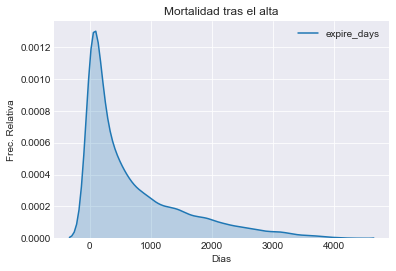
\includegraphics[scale= 0.70]{C:/mimic-iii-project/plots/Labels/expire_days.png}
\caption{Distribución de probabilidad de la mortalidad tras el alta}
\end{figure}

\begin{longtable}[]{@{}ll@{}}
\toprule
Descriptor estadístico & Valor\tabularnewline
\midrule
\endhead
Recuento & 16548 registros\tabularnewline
Media aritmética ($\mu$) & 708 dias\tabularnewline
Desviación estándar ($\sigma$) & 820 dias\tabularnewline
Valor mínimo & 0.5 dias\tabularnewline
Percentil 25\% & 88 dias\tabularnewline
Percentil 50\% & 374 dias\tabularnewline
Percentil 75\% & 1067 dias\tabularnewline
Valor máximo & 4327 dias\tabularnewline
\bottomrule
\end{longtable}

Actualmente, los estudios llevados a cabo en este campo no han sido capaces de obtener resultados clínicamente significativos mediante modelos de regresión, es decir, no ha sido posible hasta el momento obtener el valor numérico del tiempo de supervivencia de los pacientes tras su alta. Esto se debe a la gran complejidad de los datos y sus relaciones subyacentes. El trabajo en este ámbito hasta el momento se ha centrado en tareas de clasificación multiclase. De esta forma, tras explorar la información y sus estadísticas, se decide clasificar los pacientes en los siguientes tres grupos de supervivencia.

\begin{longtable}[]{@{}lll@{}}
\toprule
Mortalidad & Cantidad & Porcentaje\tabularnewline
\midrule
\endhead
12+ meses & 8391 & 37 \%\tabularnewline
1-12 meses & 6095 & 27 \%\tabularnewline
\textless{} 1 mes & 8100 & 36 \%\tabularnewline
\bottomrule
\end{longtable}

La selección se ha realizado de forma expresa para evitar clases descompensadas que dificulten la predicción posterior. Así mismo, se trata de una agrupación de utilidad en la práctica clínica. Por ejemplo, en caso de llevarse a producción el modelo y predecir que un paciente tiene altas probabilidades de morir en menos de un mes, el personal médico debería considerar la situación de este y su alta. 

Para ello, empleamos la siguiente consulta, la cual aplica directamente
la clasificación en grupos mediante una sentencia CASE en SQL.

\begin{verbatim}
SELECT hadm_id,
	CASE
		WHEN
    		EXTRACT(epoch FROM (dod-dischtime))/(3600*24*30) > 12 
    	THEN '12+ months'
    	WHEN 
    		EXTRACT(epoch FROM (dod-dischtime))/(3600*24*30) < 12 AND
     		EXTRACT(epoch FROM (dod-dischtime))/(3600*24*30) >= 1

    	THEN '1-12 months'
    									
   		WHEN
    		EXTRACT(epoch FROM (dod-dischtime))/(3600*24*30) < 1 AND
    		EXTRACT(epoch FROM (dod-dischtime))/(3600*24*30) > -0.5
    	THEN '0-1 months'	
    									
    END
AS mortality
FROM admissions a
INNER JOIN patients p
ON a.subject_id = p.subject_id
\end{verbatim}
\newpage

\section{Variables predictorias}

Tras leer biblografía, se recopilan una serie de variables que se
consideran determinantes a la hora de determinar el tiempo de
supervivencia tras el alta de la admisión hospitalaria. Las variables recopiladas se extraen a partir de consultas a la base de
datos y en algunos casos al preprocesamiento de estas. La distribución en clases atiende únicamente a criterios organizativos. 

\subsection{Información demográfica}

Se recopilan cinco variables de índole demográfica: Edad, sexo, estado
civil, religión y etnicidad. Estas variables se extraen directamente de
la tabla ADMISSIONS, excepto la edad, que se calcula a partir de la
diferencia de tiempo entre la fecha de nacimiento, almacenada en la
tabla PATIENTS, y la fecha de admisión hospitalaria, procedente de la
tabla ADMISSIONS.

\subsubsection{Edad}

La edad de los pacientes mayores a 91 años se encuentra desplazada en el
tiempo con la finalidad de proteger su identidad y dificultar su
identificación, en cumplimiento con la ley estadounidense de privacidad,
la HIPPA. De esta manera, encontramos con pacientes ancianos con edades
superiores a 300 años. Mediante una función de preprocesado substituimos
la edad de estos pacientes por 91 años. Posteriormente descartaremos
estos registros del conjunto de datos que servirá para entrenar la red
neuronal, por considerarlos poco fiables y propensos a inducir errores.
Así mismo, se descartaran igualmente los neonatos, por presentar un
comportamiento médico muy distinto al de la población adulta.
\begin{verbatim}
SELECT hadm_id, 
EXTRACT(epoch FROM (admittime dob))/(3600*24*365)
AS age
FROM admissions a
INNER JOIN patients p
ON a.subject_id = p.subject_id
\end{verbatim}

Se distribuye estadisticamente de la siguiente manera

\begin{figure}[h]
\centering
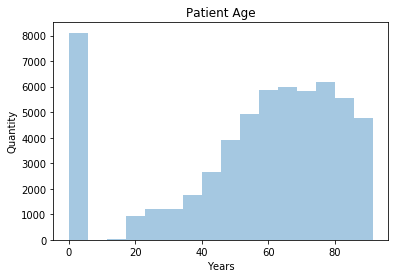
\includegraphics[scale = 0.75]{C:/mimic-iii-project/plots/Demographic_data/age_histogram.png}
\caption{Histograma de la distribución de la edad de los pacientes}
\end{figure}

\begin{longtable}[]{@{}cc@{}}
\toprule
Descriptor estadístico & Valor (años)\tabularnewline
\midrule
\endhead
Recuento & 58976\tabularnewline
Media aritmética ($\mu$) & 55.2\tabularnewline
Desviación estándar ($\sigma$) & 27.3\tabularnewline
Valor mínimo & 0\tabularnewline
Percentil 25\% & 43.5\tabularnewline
Percentil 50\% & 61.8\tabularnewline
Percentil 75\% & 75.9\tabularnewline
Valor máximo & 91.4\tabularnewline
\bottomrule
\end{longtable}

\subsubsection{Sexo}

Extraemos esta variable para cada admisión hospitalaria directamente de la base de datos, sin ningún tipo de preprocesado, mediante la siguiente consulta simple. 
\begin{verbatim}
SELECT hadm_id, gender
FROM admissions a
INNER JOIN patients p
ON a.subject_id = p.subject_id
\end{verbatim}

Se distribuye de la siguiente manera

\begin{longtable}[]{@{}lll@{}}
\toprule
 & Recuento & Proporción\tabularnewline
\midrule
\endhead
Hombres & 39250 & 55.8\% \tabularnewline
Mujeres & 26026 & 44.2\% \tabularnewline
\bottomrule
\end{longtable}

\subsubsection{Estado Civil}

Lo obtenemos mediante la siguiente consulta, de forma análoga al sexo del paciente.

\begin{verbatim}
SELECT hadm_id, marital_status
FROM admissions a
INNER JOIN patients p
ON a.subject_id = p.subject_id
\end{verbatim}
Observamos clases claramente descompensadas y poco significativas que es conveniente tratar. 

\begin{longtable}[]{@{}ll@{}}
\toprule
Estado civil & Cantidad\tabularnewline
\midrule
\endhead
DIVORCED & 3213\tabularnewline
LIFE PARTNER & 15\tabularnewline
MARRIED & 24239\tabularnewline
SEPARATED & 571\tabularnewline
SINGLE & 13254\tabularnewline
UNKNOWN (DEFAULT) & 345\tabularnewline
WIDOWED & 7211\tabularnewline
\bottomrule
\end{longtable}

Para el preprocesado de esta variable, unificamos aquellos grupos de
características similares. En concreto, se juntan los grupos DIVORCED y
SEPARATED en uno solo, y se incluye LIFE PARTNER dentro de MARRIED. Para
realizar este agrupamiento se tienen en cuenta los hábitos de vida, factores socialdemográficos y
alimentación que pueden caracterizar a cada grupo. Tras realizar esta
agrupación, llegamos a las siguientes clases:
\newpage
\begin{longtable}[]{@{}ll@{}}
\toprule
Estado civil & Cantidad\tabularnewline
\midrule
\endhead
DIVORCED/SEPARATED & 3784\tabularnewline
MARRIED & 24254\tabularnewline
SINGLE & 13254\tabularnewline
UNKNOWN & 10473\tabularnewline
WIDOWED & 7211\tabularnewline
\bottomrule
\end{longtable}


\subsubsection{Religion}
Realizamos un procedimiento análogo al llevado a cabo en la variable
MARITAL\_STATUS, teniendo en cuenta las mismas consideraciones en el
momento de unificar grupos. Extraemos la variable de la base de datos
con la siguiente consulta
\begin{verbatim}
SELECT hadm_id, religion 
FROM admissions a
INNER JOIN patients p
ON a.subject_id = p.subject_id
\end{verbatim}
De la misma manera que con el estado civil, obtenemos grupos descompensados y poco significativos. En concreto, obtenemos 20 grupos, 14 de los cuales cuentan con menos de mil registros, de un total de ~ 59k. Tras agruparlos según características culturales similares, llegamos a los siguientes grupos:
\begin{longtable}[]{@{}lc@{}}
\toprule
Religion & Valores\tabularnewline
\midrule
\endhead
BUDDHIST/HINDU & 380\tabularnewline
CHRISTIAN & 29323\tabularnewline
JEWISH/HEBREW & 5330\tabularnewline
MUSLIM & 225\tabularnewline
NONE & 23176\tabularnewline
ORTHODOX & 542\tabularnewline
\bottomrule
\end{longtable}


\subsubsection{Etnicidad}

Realizando el mismo proceso que para las variables anteriores, extraemos
y unificamos la etnicidad del paciente para cada admisión hospitalaria.

\begin{verbatim}
SELECT hadm_id, ethnicity
FROM admissions a
INNER JOIN patients p
ON a.subject_id = p.subject_id
\end{verbatim}

Se recopilan 41 orígenes étnicos distintos, algunos muy similares entre si. Por ejemplo, se hace distinción de hispanos según el país, dando lugar a numerosas categorías con menos de diez entradas. Sucede lo mismo con pacientes de origen asiático y caucásico. También hay presentes registros de pacientes con origen nativo de norteamérica (72 registros) o nativo del caribe (9 registros). Estos registros poco significativos se agrupan bajo la categoria OTHER. La agrupación realizada se puede consultar en el archivo 'mappings.py' ubicado en la carpeta resources. El resultado de preprocesar la variable es el siguiente:

\begin{longtable}[]{@{}ll@{}}
\toprule
Etnicidad & Cantidad\tabularnewline
\midrule
\endhead
ASIAN & 2007\tabularnewline
BLACK & 5785\tabularnewline
HISPANIC & 2136\tabularnewline
NONE & 5896\tabularnewline
OTHER & 1766\tabularnewline
WHITE & 41386\tabularnewline
\bottomrule
\end{longtable}

\subsection{Pruebas de laboratorio}

Se extraen diez pruebas de laboratorio comunes, realizadas
rutinariamente tras el ingreso de un paciente, para emplearlas como
variables predictorias. Para cada una de ellas, obtenemos su valor medio y su desviación
estándar, dando lugar a un total de veinte variables. Cada uno de los resultados de las pruebas se almacena en la tabla
LABEVENTS mediante un identificador, ITEMID.

La relación de ITEMIDs para las pruebas de laboratorio es la siguiente:

\begin{longtable}[]{@{}ll@{}}
\toprule
Prueba de laboratorio & ITEMID\tabularnewline
\midrule
\endhead
Nitrógeno ureico en sangre & 51066\tabularnewline
Recuento de plaquetas & 51265\tabularnewline
Hematocrito & 51221\tabularnewline
Potasio en sangre & 50971\tabularnewline
Sodio en sangre & 50983\tabularnewline
Creatinina en sangre & 50912\tabularnewline
Bicarbonato en sangre & 50882\tabularnewline
Recuento de leucocitos & 51301\tabularnewline
Glucosa en sangre & 50809, 50931\tabularnewline
Albúmina en sangre & 50862\tabularnewline
\bottomrule
\end{longtable}

Para obtener el promedio y la desviación estándar de cada una de estas
variables, por ejemplo para el sodio en sangre, realizamos la siguiente
consulta:

\begin{verbatim}
SELECT hadm_id,
avg(valuenum) AS AVG_SODIUM,
stddev(valuenum) AS STD_SODIUM,
FROM labevents
WHERE itemid = 50983
GROUP BY hadm_id
\end{verbatim}
Esta función se ejecuta en bucle para todas las pruebas de laboratorio.
En cuanto al preprocesado, descartamos aquellos valores por debajo del
percentil 1\% y por encima del percentil 99\%, al considerarlos errores
aberrantes o fallos de medicion, además de ser poco significativos. Se
realiza mediante una función creada para ello, disponible en
'preprocessing service'.

Tras extraer las variables y tratarlas, obtenemos el siguiente
resultado:



\begin{longtable}[]{@{}cccccccccc@{}}
\toprule
Prueba  & Medidas (x10\textsuperscript{3}) & $\mu$ &
$\sigma$ & mín. &  P\textsubscript{25\%} & 
 P\textsubscript{50\%} &   P\textsubscript{75\%} & máx. & Unidad \tabularnewline
\midrule
\endhead
Nitrógeno ureico & 49.9 & 24.5 & 16.1 & 5.6 & 13.4 & 19.2 &
30.3 & 93 & mg/24hr\tabularnewline
Recuento de plaquetas & 55.8 & 241.1 & 97.9 & 44.9 & 172.3 & 229 & 297.1
& 595.6 & K/uL\tabularnewline
Hematocrito & 55.9 & 33.9 & 6.9 & 23.8 & 29.1 & 31.9 & 36.7 & 58.9 &
\%\tabularnewline
Potasio en sangre & 51.8 & 4.2 & 0.4 & 3.3 & 3.9 & 4.1 & 4.4 & 5.8 &
mEq/L\tabularnewline
Sodio en sangre & 51.8 & 138.7 & 3.1 & 128.7 & 136.9 & 138.9 & 140.8 &
147.8 & mEq/L\tabularnewline
Creatinina en sangre & 49.9 & 1.3 & 1.1 & 0.35 & 0.72 & 0.93 & 1.34 &
7.9 & mg/dL\tabularnewline
Bicarbonato en sangre & 51.8 & 138.7 & 3.1 & 128.7 & 136.9 & 138.9 &
140.8 & 147.8 & mEq/L\tabularnewline
Recuento de leucocitos & 55.8 & 241 & 97.9 & 44.9 & 172.3 & 229 & 297.1
& 595.6 & K/uL\tabularnewline
Glucosa en sangre & 49.6 & 131.7 & 32.9 & 78.2 & 110 & 124.2 & 124.3 &
144.3 & mg/dL\tabularnewline
Albúmina en sangre & 30.5 & 3.2 & 0.6 & 1.7 & 2.7 & 3.2 & 3.7 & 4.7 &
g/dL\tabularnewline
\bottomrule
\end{longtable}
\subsection{Señales fisiológicas}

De la misma forma que obtenemos los resultado de las pruebas de
laboratorio, extraemos de la base de datos el promedio y la desviación
estándar de seis señales fisiológicas para emplearlas como variables
predictorias.

Las medidas han sido tomadas con dos sistemas de monitorización
distintos, Philips CareVue y Metavision. Así mismo, la base de datos
distingue entre medidas tomadas automáticamente y medidas tomadas
expresamente por el personal médico, entre otros factores. Es por ello
que una misma medida presenta múltiples identificadores.

\begin{longtable}[]{@{}ll@{}}
\toprule
Señal fisiológica & ITEMID\tabularnewline
\midrule
\endhead
Frecuencia cardíaca & 220045, 211\tabularnewline
Frecuencia respiratoria & 8113, 3603, 220210, 618\tabularnewline
Presión sistólica & 51,442,455,6701,220179,220050\tabularnewline
Presión diastólica & 8368,8440,8441,8555,220180,220051\tabularnewline
Temperatura & 223761,678\tabularnewline
Saturación de oxígeno & 646, 220277\tabularnewline
\bottomrule
\end{longtable}

Las señales fisiológicas se registran en la tabla CHARTEVENTS. Empleamos
la siguiente consulta, muy similar a la empleada para obtener los
resultados de las pruebas de laboratorio, para extraer los valores
deseados en el caso de la saturación de oxígeno.

\begin{verbatim}
SELECT hadm_id,
avg(valuenum) AS AVG_SPO2,
stddev(valuenum) AS STD_SPO2,
FROM chartevents
WHERE itemid IN (646, 220277)
GROUP BY hadm_id
\end{verbatim}

Aplicamos el mismo procesamiento usado anteriormente, es decir, descartamos aquellos valores por debajo del percentil 1\% y aquellos por encima del 99\%. La estadísticas descriptivas del promedio de estas variables se muestra en la siguiente tabla.
\begin{longtable}[]{@{}llllllllll@{}}
\toprule
Prueba  & Medidas (x10\textsuperscript{3}) & $\mu$ &
$\sigma$ & mín. &  P\textsubscript{25\%} & 
 P\textsubscript{50\%} &   P\textsubscript{75\%} & máx. & Unidad \tabularnewline
\midrule
\endhead
Frecuencia cardíaca & 55.6 & 92.2 & 22.9 & 55.5 & 78.9 & 86.8 & 99.8 &
162 & BPM\tabularnewline
Frecuencia respiratoria & 55.6 & 22.7 & 10.1 & 12.4 & 16.9 & 19.4 & 23 &
60 & BPM\tabularnewline
Presión sistólica & 48 & 120.5 & 15.2 & 86.8 & 109.2 & 118.8 & 130.6 &
163.8 & mmHg\tabularnewline
Presión diastólica & 48 & 61 & 9.7 & 39.2 & 54 & 60.1 & 67.1 & 91.8 &
mmHg\tabularnewline
Temperatura & 47.2 & 98.2 & 0.9 & 94.7 & 97.7 & 98.2 & 98.8 & 100.6 &
ºF\tabularnewline
Saturación de oxígeno & 48 & 96.9 & 1.64 & 89.3 & 96.1 & 97.2 & 98.8 &
99.8 & \%\tabularnewline
\bottomrule
\end{longtable}

\begin{figure}[h]

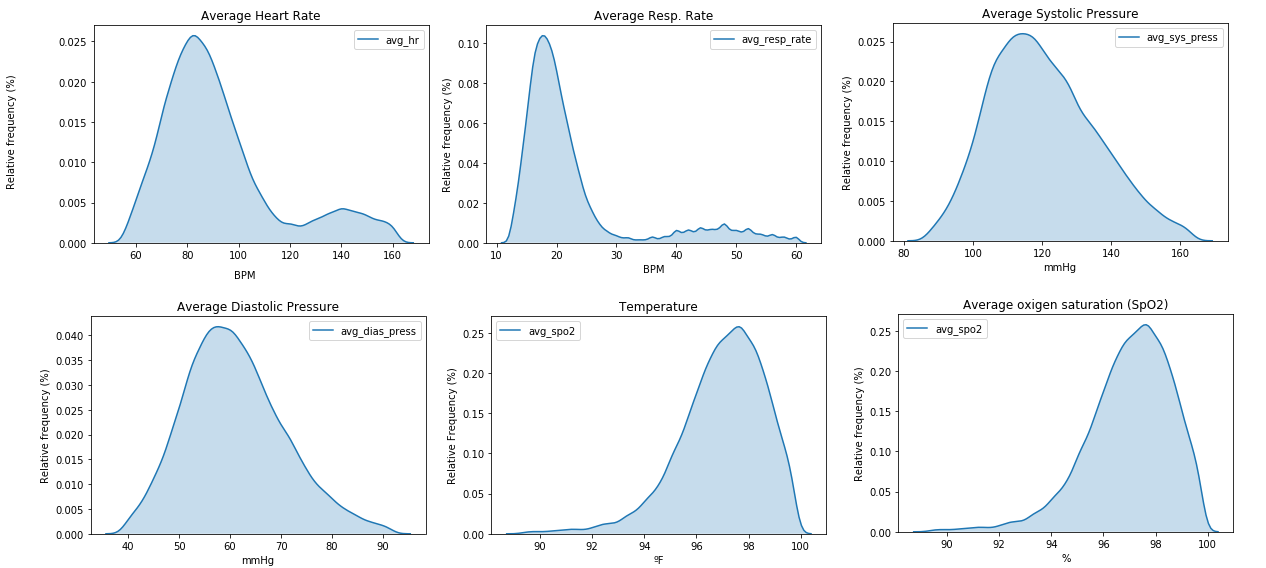
\includegraphics[width=\textwidth]{C:/mimic-iii-project/plots/Physio_data/subplot.png}
\caption{Distribución de probabilidad de las señales fisiológicas extraídas}
\end{figure}

\subsection{Información hospitalaria}

Se extraen once variables relacionadas con cada estáncia hospitalaria.

\begin{longtable}[]{@{}ll@{}}
\toprule
Variables hospitalarias & Tipo\tabularnewline
\midrule
\endhead
Servicio médico & Categórica (20 valores)\tabularnewline
Grupo de diagnóstico ICD9 & Categórica\tabularnewline
Realización de cirugía & Binaria\tabularnewline
Duración de estáncia en UCI & Numérica continua\tabularnewline
Duración de estáncia total & Numérica continua\tabularnewline
Indicador de severidad OASIS & Numérica entera\tabularnewline
Indicador de severidad SAPS & Numérica entera\tabularnewline
Indicador de severidad SOFA & Numérica entera\tabularnewline
Tiempo en ventilación mecánica & Numérica continua\tabularnewline
Fallecimiento en hospital & Binaria\tabularnewline
Cantidad de procedimientos realizados & Numéria entera\tabularnewline
\bottomrule
\end{longtable}
\paragraph{Servicio médico}
Se trata de una variable categórica que indica el servicio médico más
relevante por el cual es atendido el paciente en la estáncia
hospitalaria. Debido a que en numerosas ocasiones un paciente permanece
en más de un servicio durante su estáncia, es necesario una función de
preprocesado que extraiga el servicio de mayor importancia en función de
un criterio.

En concreto, se ha diseñado una función que utiliza la siguiente
prioridad para extraer un único servicio para cada estáncia
hospitalaria.

\begin{itemize}
\item
  Servicios de cirugía especializada 
\item
  Servicio de cirugía general
\item
  Servicio especializado
\item
  Servicio de medicina general
\end{itemize}

De esta forma, un paciente admitido en el servicio de medicina general y
posteriormente trasladado al servicio de cirugía cardíaca, constará como
un paciente tratado bajo el servicio de cirugía cardíaca únicamente, por
ejemplo. Esto permite reducir la complejidad de la variable y obtener la
información de mayor relevancia. Tras aplicar este preprocesado, se
obtienen las siguientes categorías y recuentos.

\begin{longtable}[]{@{}lll@{}}
\toprule
Servicio médico & Significado & Cantidad\tabularnewline
\midrule
\endhead
MED & Medicina general & 17260\tabularnewline
NB & Neonatos & 7806\tabularnewline
CSURG & Cirugía cardíaca & 7697\tabularnewline
CMED & Cardiología & 5860\tabularnewline
SURG & Cirugía general & 5034\tabularnewline
NSURG & Cirugía neurológica & 4024\tabularnewline
TRAUM & Traumatología & 2699\tabularnewline
NMED & Neurología & 2324\tabularnewline
OMED & Obstetricia & 1475\tabularnewline
VSURG & Cirugía vascular no cardíaca & 1371\tabularnewline
TSURG & Cirugía torácia & 1281\tabularnewline
ORTHO & Ortopédia & 739\tabularnewline
GU & Urología & 334\tabularnewline
PSURG & Cirugía plástica & 269\tabularnewline
GYN & Ginecología & 206\tabularnewline
\bottomrule
\end{longtable}

\paragraph{Grupo de diagnóstico ICD9}


ICD-9 és el acrónimo de "International Statistical Classification of
Diseases and Related Health Problems 9th Revision", publicado por la
Organización Mundial de la Salud en 1977.

Se emplean para clasificar y codificar las patólogias, lesiones,
síntomas, circustancias sociales y causas externas de enfermedades, con
el fin de recopilar información sanitaria útil relacionada con
defunciones, enfermedades y traumatismos.

Estos códigos se dividen en capítulos, secciones, categorías,
subcategorías y subclasificaciones, por ejemplo:

\newlist{myEnumerate}{enumerate}{5}
\setlist[myEnumerate,1]{label=(\arabic*)}
\setlist[myEnumerate,2]{label=(\Roman*)}
\setlist[myEnumerate,3]{label=(\Alph*)}
\setlist[myEnumerate,4]{label=(\roman*)}
\setlist[myEnumerate,5]{label=(\alph*)}


\begin{myEnumerate}
\item   Códigos 390 -- 459: Enfermededades del sistema circulatorio
    \begin{myEnumerate}
    \item Enfermedades cerebrovasculadres (430-438)
        \begin{myEnumerate}
        \item Oclusión de arterias cerebrales (434)
            \begin{myEnumerate}
            \item Embolia cerebral (434.1)
                \begin{myEnumerate}
                \item Embolia cerebral con infarto cerebral (434.1.1)
                \end{myEnumerate}
            \end{myEnumerate}
         \end{myEnumerate}
      \end{myEnumerate}
\end{myEnumerate}

La versión mas actual es la ICD-10, que se desarrolló en 1992, aunque en
la base de datos MIMIC III v1.4 se recoge la versión anterior, la ICD-9.
Actualmente, se esta realizando la transición generalizada a nivel
mundial del estándar ICD -- 9 a ICD -- 10. Debido a la gran variedad de códigos y al desbalance de clases de cada
código específico, se emplea únicamente el código primario ICD -- 9, tal
y como se recogen en el siguiente listado:

\begin{itemize}
\item
  Codigos 001 -- 139: Enfermedades infecciosas y parasitarias
\item
  Códigos 140 -- 239: Neoplasias
\item
  Códigos 240 - 279 : Enfermedades endocrinas, de la nutricion y
  metabolicas y trastornos de la inmunidad
\item
  Códigos 280 -- 289: Enfermedades de la sangre y de los órganos
  hematopoyéticos
\item
  Códigos 290 -- 319: Trastornos mentales
\item
  Códigos 320 -- 389: Enfermedades del sistema nervioso y de los órganos
  de los sentidos
\item
  Códigos 390 -- 459: Enfermedades del sistema circulatorio
\item
  Códigos 460 -- 519: Enfermedades del aparato respiratorio
\item
  Códigos 520 -- 579: Enfermedades del aparato digestivo
\item
  Códigos 580 -- 629: Enfermedades del aparato genitourinario
\item
  Códigos 630 -- 679: Complicaciones del embarazo, parto y puerperio
\item
  Códigos 680 -- 709: Enfermedades de la piel y del tejido subcutáneo
\item
  Códigos 710 -- 739: Enfermedades del sistema osteo-mioarticular y
  tejido conjuntivo
\item
  Códigos 740 -- 759: Anomalías congénitas
\item
  Códigos 760 -- 779: Ciertas enfermedades con origen en el periodo
  perinatal
\item
  Códigos 780 -- 799: Síntomas, signos y estados mal definidos
\item
  Códigos 800 -- 999: Lesiones y envenenamientos
\item
  Códigos E y V: Causas externas de lesiones y clasificación
  suplementaria. 
\end{itemize}

Mediante la siguiente consulta obtenemos el código ICD-9 de mayor
prioridad para cada admisión, indicado por seq\_num = 1 en la base de datos.

\begin{verbatim}
SELECT hadm_id, diagnoses_icd.icd9_code
FROM diagnoses_icd  
INNER JOIN d_icd_diagnoses 
ON diagnoses_icd.icd9_code = d_icd_diagnoses.icd9_code 
WHERE seq_num = 1
\end{verbatim}

Es necesaria una función de filtrado que convierta el código ICD-9
específico a su clasificación mayor en función de su número de código,
lo cual se realizará en la etapa de preprocesado.

\paragraph{Realización de cirugía}

Para detectar si se han realizado intervenciones quirúrgicas en un
paciente durante su estancia hospitalaria emplearemos los indicadores de
cirugía, (Surgery Flags), proporcionados por el HCUP, Healthcare Cost
and Utilization Project, una iniciativa financiada por el gobierno
estadounidense mediante la `Agency for Healthcare Research and Quality'
(AHRQ) dedicada a la gestión y análisis de datos médicos.

Esta entidad proporciona herramientas para identificar intervenciones y
eventos quirúrgicos mediante códigos ICD-9 de procemiento o códigos CPT
(Current Procedural Terminology) , ambos presentes en la base de datos
MIMIC-III v.1.4.

Permite la clasificación de procedimientos en tres grupos:

\begin{itemize}
\item
  NARROW: Procedimientos quirúrgicos terapéuticos invasivos requiriendo
  incisión, extirpación, manipulación o suturado de tejido que penetra o
  atraviesa la piel, típicamente se realiza en quirófano y con anestesia
  local o general o sedación.
\item
  BROAD: Procedimientos quirúrgicos que no se pueden clasificar como
  aquellos incluidos en el indicador NARROW, pero se realizan bajo
  condiciones quirúrgicas. Este grupo incluye procedimientos quirúrgicos
  de diagnóstico, como procedimientos endoscópicos o percutáneos, o
  aquellos realizados a través de orificios naturales. Se trata de
  intervenciones menos invasivas.
\item
  NEITHER: Procedimientos no registrado como NARROW o BROAD, es decir,
  procedimientos no quirúrgicos. 
\end{itemize}

Esta clasificación se distribuye en forma de archivo CSV y mediante
Python se diseña una función para devolver la clasificación del
procedimiento.

Debido a que unicamente se clasifican un 4\% de registros como BROAD, se
decide incluir estos dentro de NARROW con el fin de evitar clases
desproporcionadas, dando lugar a una variable binaria con la siguiente
distribución.

\begin{longtable}[]{@{}ccc@{}}
\toprule
Indicador de cirugía & Recuento & Porcentaje\tabularnewline
\midrule
\endhead
Narrow & 29867 & 56\%\tabularnewline
No Surgery & 23043 & 44\%\tabularnewline
\bottomrule
\end{longtable}
\newpage
\paragraph{Duración de estancia en UCI}
De la base de datos es posible extraer directamente la duración de
estancia en UCI en dias para cada paciente en una misma admisión
hospitalaria. Esta información se haya en la tabla ICUSTAYS y la
obtenemos mediante la siguiente consulta.

\begin{verbatim}
SELECT hadm_id, 
sum(los) AS total_icu_time 
FROM icustays
GROUP BY hadm_id
\end{verbatim}

Es necesario emplear la función agregada de suma en la consulta debido a
que en ciertas ocasiones un paciente ingresa en la UCI, es transferido a
otra sección y posteriormente regresa a la UCI, con lo cual se registran
distintas duraciones para una misma estancia. De esta forma, obtenemos
una variable continua, a la cual no aplicamos preprocesado.


\begin{figure}[h]
\centering
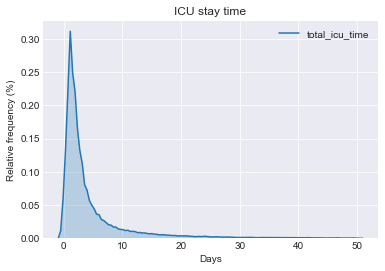
\includegraphics[scale = 0.70]{C:/mimic-iii-project/plots/ICU_data/icu_time.png}
\caption{Distribución de probabilidad de la estáncia en UCI}
\end{figure}
\newpage

\paragraph{Duración de estáncia hospitalaria}

Obtenemos la duración de estáncia hospitalaria, incluyendo la duración
en UCI, como la diferencia entre el tiempo de admisión y de alta. Para
ello empleamos la función EXTRACT y epoch, propias de PostgreSQL.

\begin{verbatim}
SELECT hadm_id, 
EXTRACT(epoch FROM(dischtime - admittime))/(3600*24) AS total_los_days
FROM admissions
\end{verbatim}
Esta variable se mide también en dias y no requiere preprocesado. Se distribuye de la siguiente manera.

\begin{figure}[h]
\centering
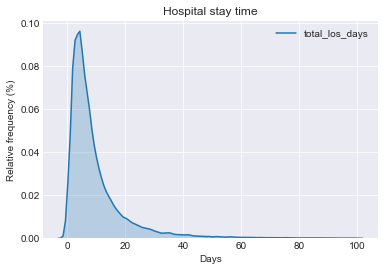
\includegraphics[scale = 0.70]{C:/mimic-iii-project/plots/ICU_data/los_time.png}
\caption{Distribución de probabilidad de la estáncia hospitalaria completa}
\end{figure}

\paragraph{Recuento de admisiones}

Para cada admisión, indica la cantidad de estancias hospitalarias que ha
realizado el mismo paciente, contando también la misma. Esto permite identificar aquellas admisiones correspondientes a
pacientes readmitidos en diversas ocasiones, lo cual puede ser indicador
de sujetos con enfermedades crónicas, que requieren regularmente
atención médica. Obtenemos esta variable mediante funciones de preprocesado sobre la
tabla ADMISSIONS.


\paragraph{Recuento de procedimientos}
Indica la cantidad de procedimientos, tanto quirúrgicos como no
quirúrgicos, realizados a un paciente en una misma estancia
hospitalaria. Se trata de una variable numérica discreta que obtenemos
mediante la siguiente consulta.

\begin{verbatim}
SELECT hadm_id, count(*) AS procedure_count
FROM procedures_icd
GROUP BY hadm_id
\end{verbatim}
Esta variable no requiere de preprocesado.

\paragraph{Tiempo en ventilación mecánica}

Empleando de nuevo una vista materializada disponible en el repositorio
de código de MIMIC-III, obtenemos el tiempo que pasa cada paciente en
ventilación mecánica durante su estáncia hospitalaria. Utilizamos la
siguiente consulta sobre la vista VENTDURATIONS.

\begin{verbatim}
SELECT hadm_id, SUM(duration_hours) AS total_mech_vent_time
FROM ventdurations v
INNER JOIN icustays i
ON v.icustay_id = i.icustay_id
GROUP BY hadm_id
\end{verbatim}
En ocasiones, un paciente pasa un tiempo conectado al ventilador
mecánico, es desconectado, y conectado de nuevo posteriormente. Es por
ello que la vista materializada registra en ocasiones diversas entradas
para una misma estancia en UCI, con lo cual es conveniente calcular la
suma de duraciones para una estancia.

\subsubsection{Indicadores de severidad}
Distintos indicadores de severidad han sido desarrollados con el
objetivo y predecir la mortalidad hospitalaria a partir de la
información de los pacientes, en particular de las medidas tomadas
durante las primeras 24h horas de su ingreso. Sin embargo, presentan
ciertas limitaciones, por ejemplo al depender de medidas subjetivas
tomadas por el personal médico o al emplear relaciones lineales que no
se adaptan a la realidad.

Utilizaremos como variables predictoras los indicadores SOFA, SAPS y
OASIS, los cuales obtendremos mediante la siguiente consulta:

\begin{verbatim}
SELECT o.hadm_id, 
AVG(o.oasis) AS oasis_avg, 
AVG(so.sofa) AS sofa_avg, 
AVG(sa.saps) as saps_avg
FROM oasis o
INNER JOIN sofa so
ON o.hadm_id = so.hadm_id
INNER JOIN saps sa
ON sa.hadm_id = so.hadm_id
GROUP BY o.hadm_id
\end{verbatim}

Para obtener estos indicadores, utilizamos scripts del repositorio de
código oficial de MIMIC-III.
{[}https://github.com/MIT-LCP/mimic-code/tree/master/concepts/severityscores{]}.
De esta manera, creamos vistas materializadas que contienen los
indicadores de severidad precalculados para cada admision hospitalaria.

\paragraph{SOFA}

``Sequential Organ Failure Assessment score''. Creado en 1994 por la
European Society of Intensive Medicine (ESICM), este indicador fue
desarrollado para evaluar la severidad de la enfermedad del paciente,
basada en el grado de fallo orgánico de seis órganos. En concreto, se
toman las siguientes medidas.

\begin{itemize}
\item
  Sistema respiratorio:
\item
  \begin{itemize}
  \item
    PaO2
  \item
    Presencia de ventilación mecánica
  \end{itemize}
\item
  Sistema nervioso:
\item
  \begin{itemize}
  \item
    Glasgow Coma Scale. 
  \end{itemize}
\item
  Sistema cardiovascular:
\item
  \begin{itemize}
  \item
    Presión arterial media
  \item
    Nivel de dopamina
  \item
    Nvel de Epinefrina
  \item
    Nivel de norepinefrina
  \end{itemize}
\item
  Hígado:
\item
  \begin{itemize}
  \item
    Nivel de bilirrubina
  \end{itemize}
\item
  Coagulación:
\item
  \begin{itemize}
  \item
    Nivel de plaquetas
  \end{itemize}
\item
  Renal:
\item
  \begin{itemize}
  \item
    Nivel de creatinina
  \item
    Volumen de orina
  \end{itemize}
\end{itemize}

Los resultados de estas pruebas otorgan puntuaciones entre 0 y 4, que
posteriormente se suman para obtener la puntuación SOFA total. Permite
obtener una idea aproximada de la mortalidad del paciente, de manera
sencilla y directa de calcular a partir de solamente once variables
básicas.
\paragraph{SAPS}

Simplified Acute Physiology Score. Creado en 1993 por Le Gall y
Lemenshow Saulnier, se emplea para medir la severidad de la enfermedad
de los paciente admitidos en unidad de cuidados intensivos de edad mayor
a 15 años. Se completa 24h tras el ingreso y otorga una puntuación de
entre 0 y 163, además de la mortalidad predecida en porcentaje. Se
calcula a partir de 12 medidas fisiológicas básicas, la edad del
paciente y el tipo de admisión.

El resultado de SAPS es mejor empleado para contrastar la gravedad de
grupos de pacientes con patologías distintas, más que a nivel
individual, debido a que sus resultados pueden ser poco precisos a nivel
de paciente.

\paragraph{OASIS}

OASIS, Oxford Acute Severity of Illness Score, se trata de un indicador
de severidad diseñado en 2013 por Johnson AE1, Kramer AA, Clifford GD,
de la Universidad de Oxford. Se caracteriza por emplear técnicas de
aprendizaje automático, en concreto optimización por enjambre de
partículas, y por no requerir un gran trabajo de recolección de
información, ya que requiere unicamente diez características, excluyendo
medidas de laboratorio, o informacion sobre diagnósticos y
comorbilidades.

\paragraph{Escala de coma de Glasgow}

Se trata de una escala neurológica diseñada para medir facilmente y de
forma objetiva el estado de cosciencia de una persona. Un paciente es
puntuado segun unos criterios en diversos aspectos, y la suma de
puntuaciones otorga una puntuación entre 3, indicando profunda
inconsciencia, y 14, indicando un estado de alerta normal.

Se emplea también como variable para calcular los indicadores de
severidad OASIS, SAPS y SOFA. Se calcula siguiendo los criterios
siguientes:

\begin{figure}[h]
\centering
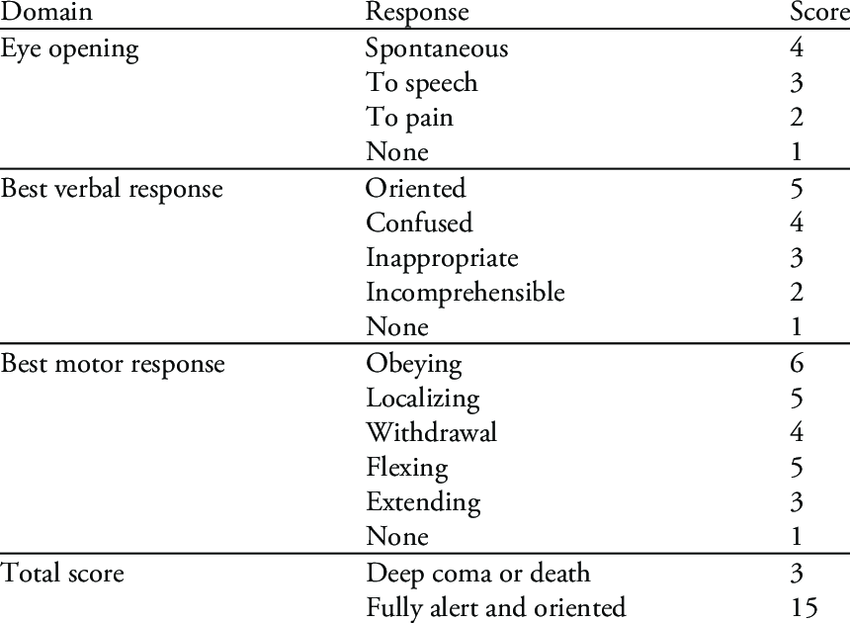
\includegraphics[scale = 0.30]{C:/mimic-iii-project/plots/glasgow_coma_scale.png}
\caption{Parámetros para calcular el valor de coma de Glasgow}
\end{figure}

\paragraph{Tiempo en ventilación mecánica}
Empleando de nuevo una vista materializada disponible en el repositorio
de código de MIMIC-III, obtenemos el tiempo que pasa cada paciente en
ventilación mecánica durante su estáncia hospitalaria. Utilizamos la
siguiente consulta sobre la vista VENTDURATIONS.

\begin{verbatim}
SELECT hadm_id, SUM(duration_hours) AS total_mech_vent_time
FROM ventdurations v
INNER JOIN icustays i
ON v.icustay_id = i.icustay_id
GROUP BY hadm_id
\end{verbatim}

En ocasiones, un paciente pasa un tiempo conectado al ventilador
mecánico, es desconectado, y conectado de nuevo posteriormente. Es por
ello que la vista materializada registra en ocasiones diversas entradas
para una misma estancia en UCI, con lo cual es conveniente calcular la
suma de duraciones para una estancia.

\end{document}

